\documentclass[11pt,respuestas,a4]{aleph-examen}
%\documentclass[11pt,a4]{aleph-examen}
% Se puede ver la documentación aquí: 
% https://github.com/alephsub0/LaTeX_aleph-examen

% -- Paquetes adicionales 
\usepackage{aleph-comandos}
\usepackage{booktabs}
\usepackage{multicol}
\usepackage{pgfplots}
\usetikzlibrary{intersections, pgfplots.fillbetween}
% -- Datos 
\institucion{Escuela de Ciencias Físicas y Matemática}
\carrera{Medicina Veterinaria}
\asignatura{Matemática I*}
\tema{Examen escrito no. 3}
\autor{Fernando Jiménez T.}
\fecha{Semestre 2024-2}


\logouno[0.14\textwidth]{Logos/logoPUCE_04_ac}
\definecolor{colortext}{HTML}{0030A1}
\definecolor{colordef}{HTML}{0030A1}
\fuente{montserrat}


\begin{document}

\encabezado

\section*{Indicaciones}
\begin{itemize}[leftmargin=*]
\item 
    En esta actividad se evalúa si el estudiante \textit{(Criterio 3.2) evaluará la capacidad de plantar ecuaciones e inecuaciones, resolverlas y analizar las soluciones obtenidas, verificando su validez y pertinencia en problemas prácticos.} 
\item
    Se encuentra prohibido el uso de cualquier fuente de información durante todo el examen.
\item
    En caso de considerar que existe un error en la pregunta o que esta se encuentra mal planteada, se debe indicar cuál es el error y justificarlo.
\item
    Todas las soluciones deben estar correctamente redactadas y explicadas.
\end{itemize}

\section*{Ejercicios}

\begin{preguntas}

%%%%%%%%%%%%%%%%%%%%%%%%%%%%%%%%%%%%%%%%
\item Colorear el \'area soluci\'on de los siguientes sistemas de desigualdades en los gr\'aficos dados. \puntaje{10 }
\begin{multicols}{2}
	\begin{enumerate}[label=\textit{\alph*)}]
		\item $\begin{cases}
			x - y  \leq 0 \\
			x + y \geq 2
		\end{cases}$
		\begin{flushleft}
			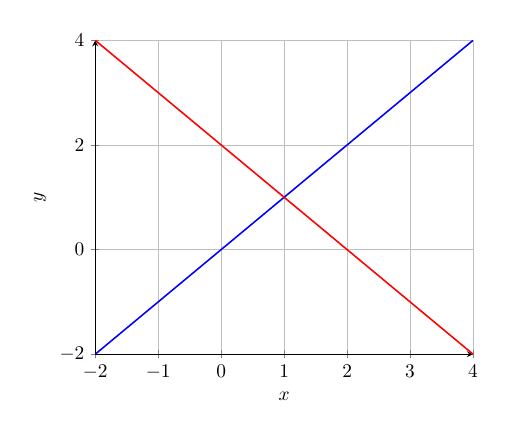
\begin{tikzpicture}[scale=0.7]
				\begin{axis}[
					axis lines = left,
					xlabel = {$x$},
					ylabel = {$y$},
					ymin=-2, ymax=4, xmin=-2, xmax=4,
					grid=both,
					domain=-2:4,
					samples=100
					]
					\addplot[color=blue, thick]{x};
					\addplot[color=red, thick]{2-x};
				\end{axis}
			\end{tikzpicture}
		\end{flushleft}
		\item $\begin{cases}
			x - y  \geq 0 \\
			x + y \leq 2
		\end{cases}$
		\begin{flushleft}
			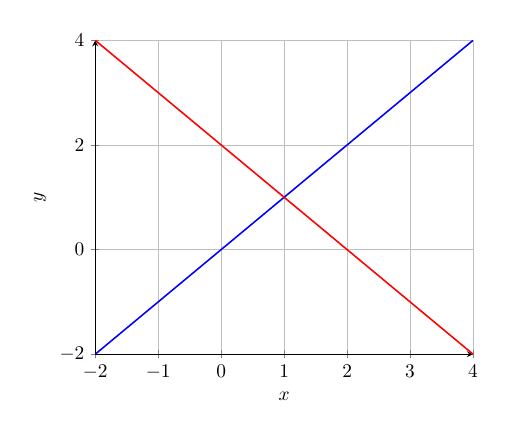
\begin{tikzpicture}[scale=0.7]
				\begin{axis}[
					axis lines = left,
					xlabel = {$x$},
					ylabel = {$y$},
					ymin=-2, ymax=4, xmin=-2, xmax=4,
					grid=both,
					domain=-2:4,
					samples=100
					]
					\addplot[color=blue, thick]{x};
					\addplot[color=red, thick]{2-x};
				\end{axis}
			\end{tikzpicture}
		\end{flushleft}
	\end{enumerate}
\end{multicols}
% -----------------------------
\begin{respuesta}
\begin{multicols}{2}
	\begin{enumerate}[label=\textit{\alph*)}]
		\item $\begin{cases}
			x - y  \leq 0 \\
			x + y \geq 2
		\end{cases}$
		\begin{flushleft} 
			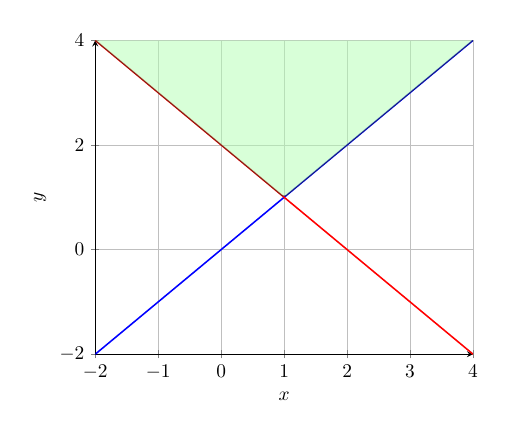
\begin{tikzpicture}[scale=0.7] 
				\begin{axis}[
					axis lines = left,
					xlabel = {$x$},
					ylabel = {$y$},
					ymin=-2, ymax=4, xmin=-2, xmax=4,
					grid=both,
					domain=-2:4,
					samples=100
					]
					\addplot[color=blue, thick]{x};
					\addplot[color=red, thick]{2-x};
					\addplot [fill=green!30,  opacity=0.5, domain=-2:4 ]{max(x, 2-x)};
				\end{axis}
			\end{tikzpicture}
		\end{flushleft}
		\item $\begin{cases}
			x - y  \geq 0 \\
			x + y \leq 2
		\end{cases}$
		\begin{flushleft}
			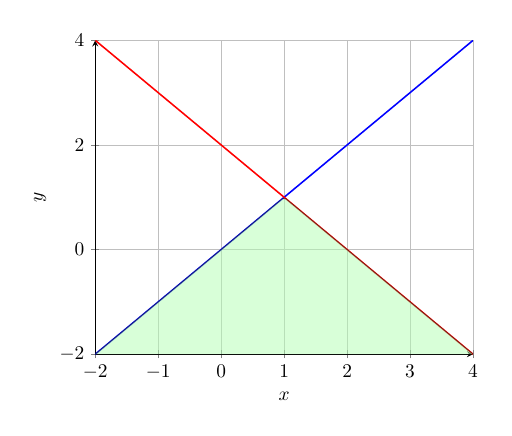
\begin{tikzpicture}[scale=0.7]
				\begin{axis}[
					axis lines = left,
					xlabel = {$x$},
					ylabel = {$y$},
					ymin=-2, ymax=4, xmin=-2, xmax=4,
					grid=both,
					domain=-2:4,
					samples=100
					]
					\addplot[color=blue, thick]{x};
					\addplot[color=red, thick]{2-x};
					\addplot [fill=green!30,  opacity=0.5, domain=-2:4 ]{min(x, 2-x)};
				\end{axis}
			\end{tikzpicture}
		\end{flushleft}
	\end{enumerate}
\end{multicols}
\end{respuesta}
%%%%%%%%%%%%%%%%%%%%%%%%%%%%%%%%%%%%%%%%
\item Graficar la soluci\'on de los siguientes sistemas de desigualdades: \puntaje{20}
\begin{multicols}{2}
    \begin{enumerate}[label=\textit{\alph*)}]
        \item $\begin{cases}
        	x+y \leq 4 \\
        	-x + y \geq 0
        \end{cases}$
        \item $\begin{cases}
        	x -y > 0 \\
        	-2x + y \leq -4 
        \end{cases}$
    \end{enumerate}
\end{multicols}
% -----------------------------
\begin{respuesta}
\begin{multicols}{2}
    \begin{enumerate}[label=\textit{\alph*)}]
        \item  \hspace{1cm}
        
        \begin{flushleft}
        	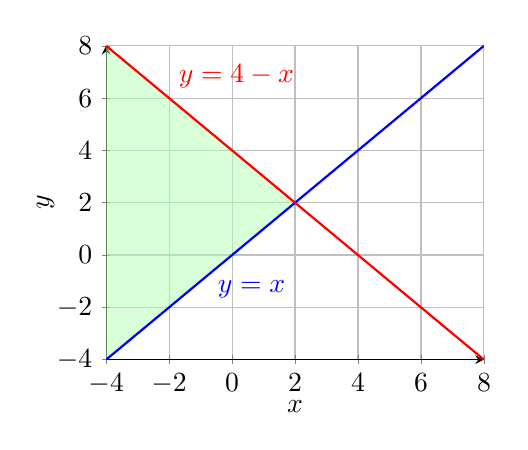
\begin{tikzpicture}[scale=0.7]
        		\begin{axis}[
        			axis lines = left,
        			xlabel = {$x$},
        			ylabel = {$y$},
        			ymin=-4, ymax=8, xmin=-4, xmax=8,
        			grid=both,
        			domain=-4:8,
        			samples=100
        			]
        			\addplot[name path = A, color=blue, thick]{x};
        			\addplot[name path = B, color=red, thick]{4-x};
        			\addplot [green!30, opacity = 0.5] fill between [of = A and B, soft clip={domain=-4:2}];
        			
        			\node at (axis cs: 2, -2) [anchor=south east] {\textcolor{blue}{$y = x$}};
        			\node at (axis cs: -2, 6) [anchor=south west] {\textcolor{red}{$y = 4 - x$}};
        		\end{axis}
        	\end{tikzpicture}
        \end{flushleft}
        % -------------
        \item \hspace{1cm}
        
        \begin{flushleft}
        	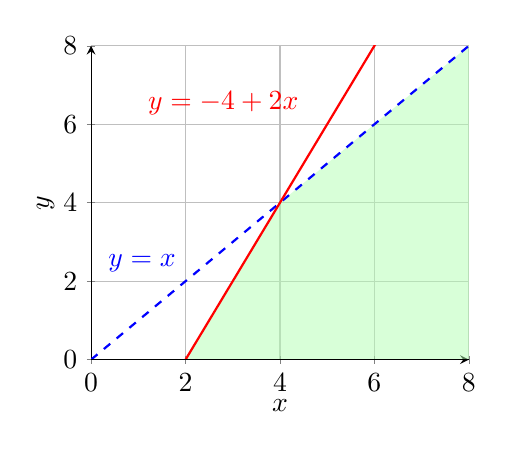
\begin{tikzpicture}[scale=0.7]
        		\begin{axis}[
        			axis lines = left,
        			xlabel = {$x$},
        			ylabel = {$y$},
        			ymin=0, ymax=8, xmin=0, xmax=8,
        			grid=both,
        			domain=0:8,
        			samples=100
        			]
        			\addplot[name path = A, color=blue, thick, dashed]{x};
        			\addplot[name path = B, color=red, thick]{-4+2*x};
        			\addplot[name path = C, color=black, thick]{0};
        			\addplot [green!30, opacity = 0.5] fill between [of = C and B, soft clip={domain=2:4}];
        			\addplot [green!30, opacity = 0.5] fill between [of = C and A, soft clip={domain=4:8}];
        			
        			\node at (axis cs: 2, 2) [anchor=south east] {\textcolor{blue}{$y = x$}};
        			\node at (axis cs: 1, 6) [anchor=south west] {\textcolor{red}{$y = -4 + 2x$}};
        		\end{axis}
        	\end{tikzpicture}
        \end{flushleft}
    \end{enumerate}
\end{multicols}
\end{respuesta}
%%%%%%%%%%%%%%%%%%%%%%%%%%%%%
\item Una investigadora realiza un experimento para probar una hipótesis donde intervienen los nutrientes niacina y retinol. Ella alimenta a un grupo de ratas de laboratorio con una dieta diaria de precisamente 32 unidades de niacina y 22 mil unidades de retinol. Ella usa dos tipos de alimentos comerciales en forma de pastillas. El alimento A contiene 0.12 unidades de niacina y 100 unidades de retinol por gramo; el alimento B contiene 0.20 unidades de niacina y 50 unidades de retinol por gramo.

¿Cuántos gramos de cada alimento les da ella al grupo de ratas diariamente? \puntaje{15}
% -----------------------------
\begin{respuesta}
	Definamos las variables:
	\begin{itemize}
		\item[] $x$ es la cantidad en gramos del alimento $A$.
		\item[] $y$ es la cantidad en gramos del alimento $B$.
	\end{itemize}
	La primera ecuaci\'on nos dice la cantidad total de niacina que se obtuvo al mezclar ambos alimentos, es decir,
	$$
	0.12 x + 0.20 y = 32
	$$
	La segunda ecuaci\'on nos dice la cantidad total de retinol que se obtiene al mezclar los alimentos.
	$$
	100 x + 50 y = 22 000
	$$
	Es decir, el sistema que debemos resolver es:
	$$
	\begin{cases}
		0.12 x + 0.20 y = 32 \\
		100 x + 50 y = 22 000
	\end{cases}
	$$
	Un sistema equivalente se obtiene al multiplicar por 100 a la primera restricci\'on, obteniendo:
	$$
	\begin{cases}
		12 x + 20 y = 3200 \\
		100 x + 50 y = 22 000
	\end{cases}
	$$
	Despejando $y$ de la primera restricci\'on obtenemos:
	$$
	y = \frac{3200 - 12x }{20}
	$$
	Reemplazando el valor de $y$ en la segunda restricci\'on tenemos:
	$$
	100 x + 50 \left( \frac{3200 - 12x }{20} \right) = 22000
	$$
	Resolviendo esta ecuaci\'on lineal tenemos:
	$$
	x = 200
	$$
	Reemplazando el valor de $x = 200$ en la la ecuaci\'on $y = \frac{3200 - 12x}{20}$, tenemos
	$$
	y = 40
	$$
	La investigadora ha usado 200 gramos del alimento A y 40 gramos del alimento B para alimentar a las ratas.
\end{respuesta}
% -----------------------------
\end{preguntas}
\end{document}